
\documentclass[12pt]{article}
\title{ECE 141 Homework 4}
\usepackage{subcaption}
\author{Lawrence Liu}
\usepackage{graphicx}
\usepackage{amsmath}
\usepackage{placeins}
\newcommand{\Laplace}{\mathscr{L}}
\setlength{\parskip}{\baselineskip}%
\setlength{\parindent}{0pt}%
\usepackage{xcolor}
\usepackage{listings}
\definecolor{backcolour}{rgb}{0.95,0.95,0.92}
\usepackage{amssymb}
\lstdefinestyle{mystyle}{
    backgroundcolor=\color{backcolour}}
\lstset{style=mystyle}

\begin{document}
\maketitle
\subsection*{Problem 5.9}
The transfer function is $$\frac{Y}{R}=\frac{5}{(s(s+2)+5+5\alpha s)}$$, therefore the characteristic equation is $s(s+2)+5+5\alpha s=0$, therefore we have $b(s)=5s$ and $a(s)=s^2+2s+1$
Therefore we have that $L(s)=\frac{5s}{s^2+2s+1}$, therefore 1 line will approach asymptotes centered at $-2$ and leaving at angles $180^{\circ}$. Furthermore, the departure angle from the poles
$-1\pm 2j$ is $\mp153.4^{\circ}$ and the arival angle to the zero at 0 is $180^{\circ}$, therefore the root locuses are at 
\\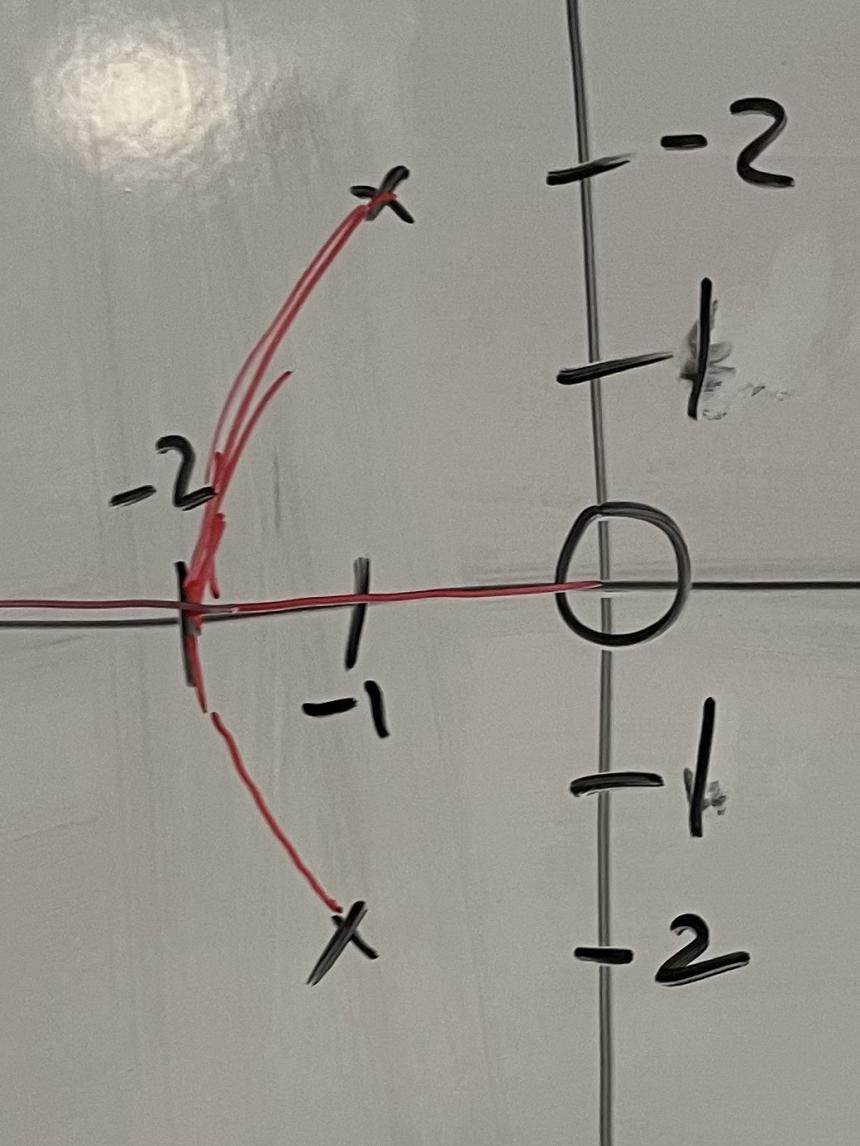
\includegraphics[scale=0.25]{Problem1fig1.jpg}\\
When $\alpha=0$, there are poles at $-1\pm 2j$, when $\alpha=0.5$, there are poles at $-2$ and $-2.5$, and when $\alpha=2$, there are poles at $-0.432$ and $-11.568$, therefore the plot of the poles looks like
\\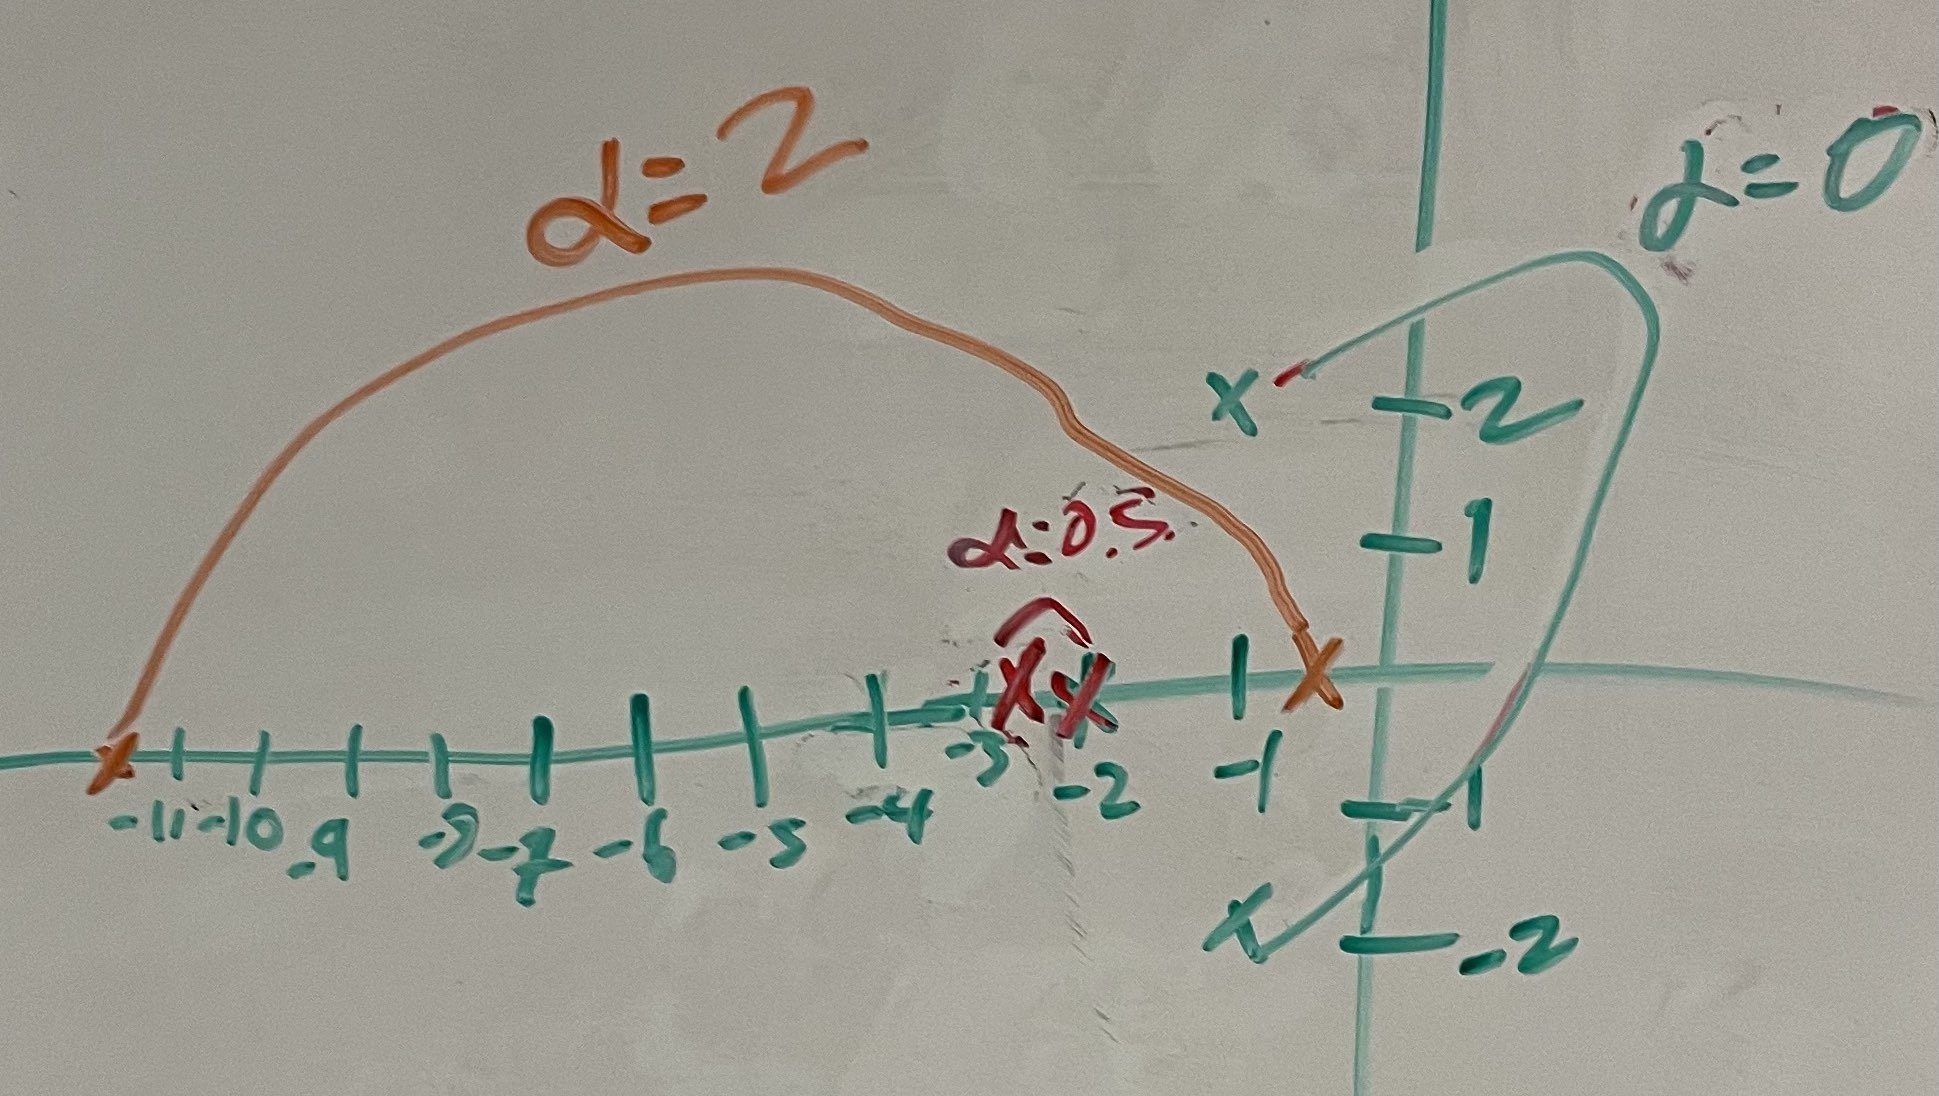
\includegraphics[scale=0.15]{Problem1fig2.jpg}\\
Therefore since $alpha=0$ the step response will be underdamped since it has poles with imaginary components, and for $\alpha=0.5$ the damping factor $\zeta=\frac{4.5}{2\sqrt{5}}$ and when 
$\alpha=2$ the damping factor $\zeta=\frac{6}{\sqrt{5}}$, therefore the plot of the step responses would look like
\\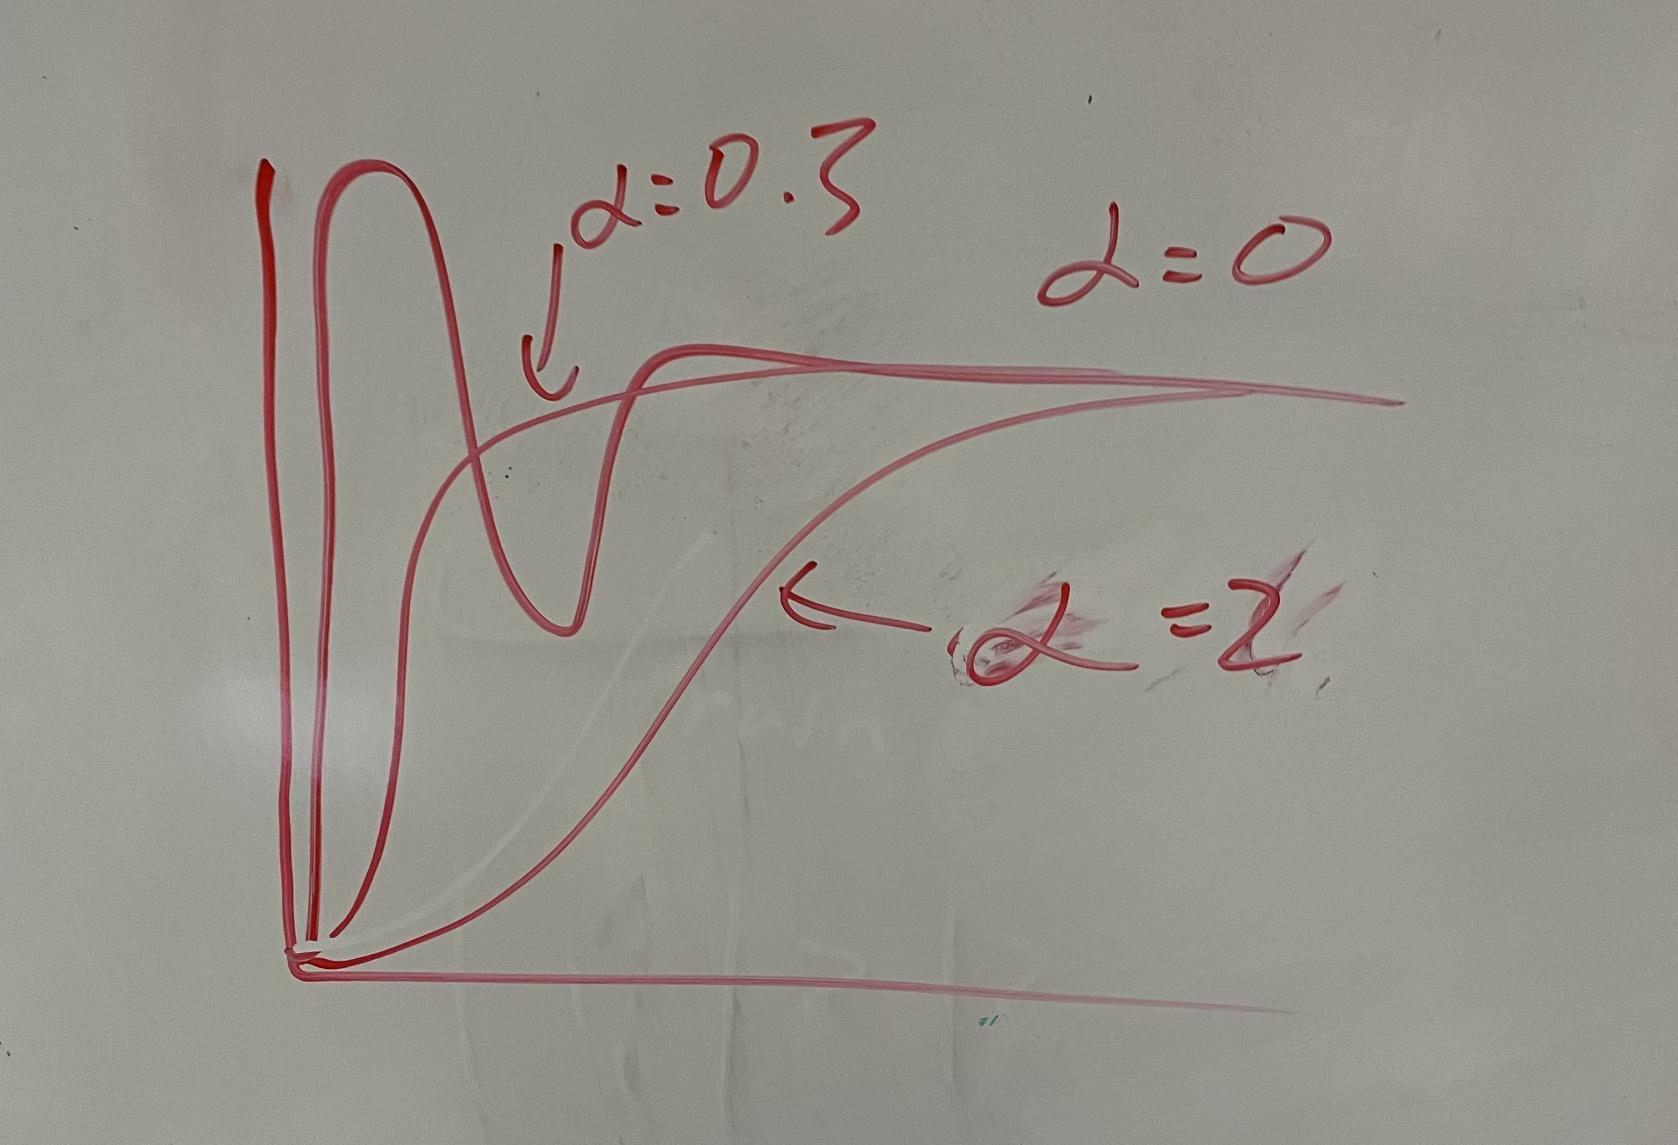
\includegraphics[scale=0.15]{Problem1fig3.jpg}\\
With the following matlab code we can verify it
\begin{verbatim}
sys = tf([5],[1 2 5]);
step(sys)
stepinfo(sys)
hold on;

sys = tf([5],[1 2+2.5 5]);
step(sys)
stepinfo(sys)

sys = tf([5],[1 12 5]);
step(sys)
stepinfo(sys)

hold off;
legend('alpha=0','alpha=0.5','alpha=2')
\end{verbatim}
Which produces the following plot.\\
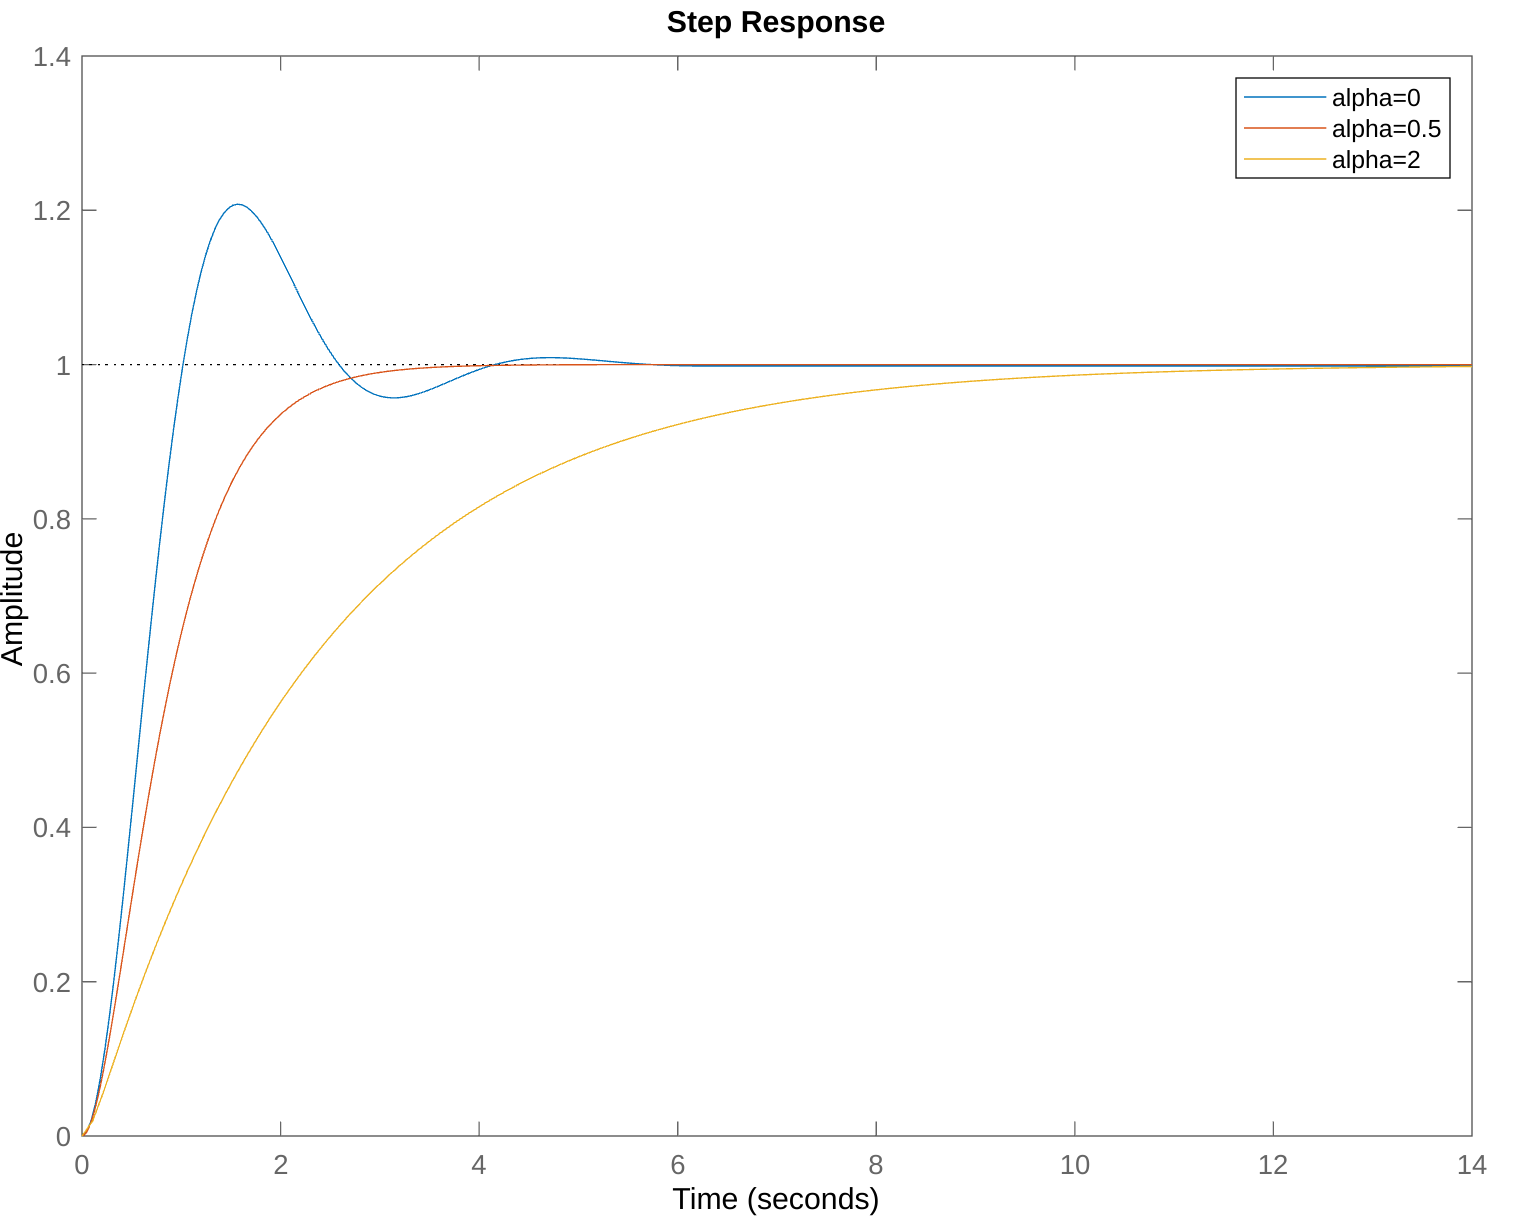
\includegraphics[scale=0.25]{Problem1fig4.png}\\
\section*{Problem 5.13}
\subsection*{(a)}
The transfer function is $\frac{K\frac{(s+1)(s^2+81)}{(s+13)s^2(s+100)}}{1+K\frac{(s+1)(s^2+81)}{(s+13)s^2(s+100)}}$, therefor $L(s)=\frac{(s+1)(s^2+81)}{(s+13)s^2(s+100)}$
and therefore with the following matlab code we can get that the Roots Locus looks like 
\begin{verbatim}
sys = tf([1 1 81 81],[1 13 100 1300 0 0]);
rlocus(sys)
\end{verbatim}
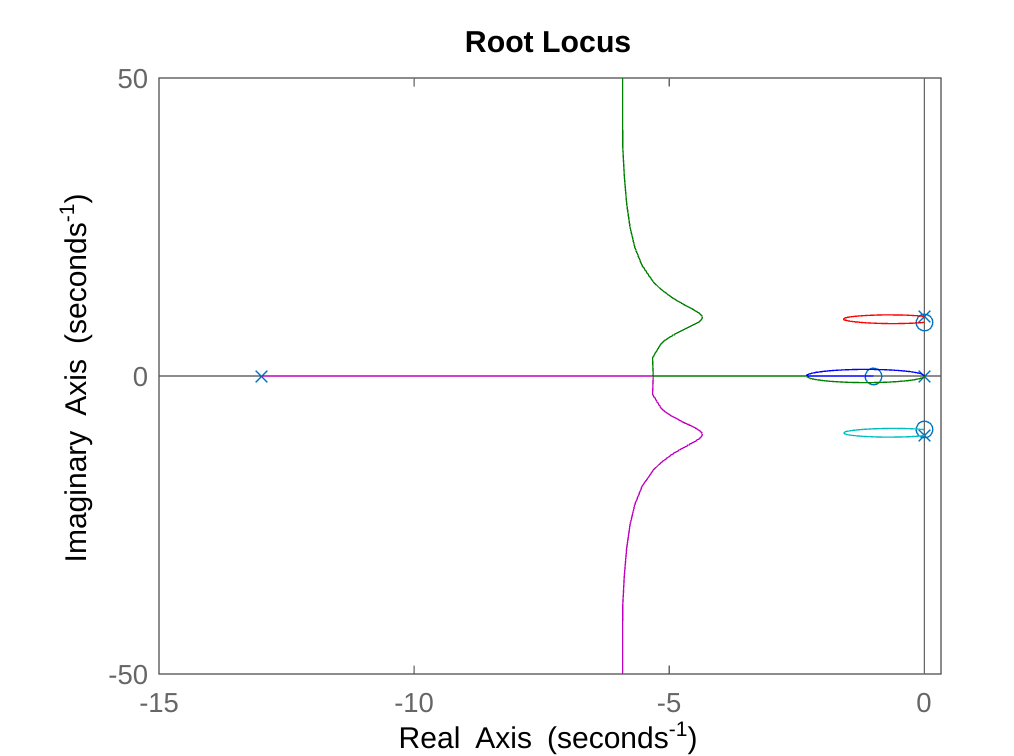
\includegraphics[scale=0.25]{Problem2Fig1.png}\\
\subsection*{(b)}
No there isn't, we can confirm this through the following matlab code
\begin{verbatim}
sys = tf([1 1 81 81],[1 13 100 1300 0 0]);
[r,k] = rlocus(sys);
phases=atan2(imag(r),real(r));
sum(sum(phases>0.5==5))
\end{verbatim}
The outputs 0, so there is no values of $K$ such that all roots have a damping factor $\zeta>0.5$
\subsection*{(c)}
From the following code we get that the possible values of $K$ are $K=32.6$ and $K=88.3$
\begin{verbatim}
syms s

sys = tf([1 1 81 81],[1 13 100 1300 0 0]);
thresh=0.001;
zeta=0.707;
L=50;
plot([-zeta*L 0 -zeta*L],[-sqrt(1-zeta^2)*L 0 sqrt(1-zeta^2)*L])
hold on;
k = (20:0.1:40);
r = rlocus(sys,k);
rlocus(sys)
phases=atan2(-real(r),abs(imag(r)));
loc=sum((abs(phases-0.786)<thresh))==2;
Gain=k(loc)

plot(real(r(:,loc)),imag(r(:,loc)),'b*')

k = (80:0.1:120);
r = rlocus(sys,k);
rlocus(sys)
phases=atan2(-real(r),abs(imag(r)));
loc=sum((abs(phases-0.786)<thresh))==2;
Gain=k(loc)

plot(real(r(:,loc)),imag(r(:,loc)),'b+')
hold off;
xlim([-15 0])
\end{verbatim}
Which also produces the following graph\\
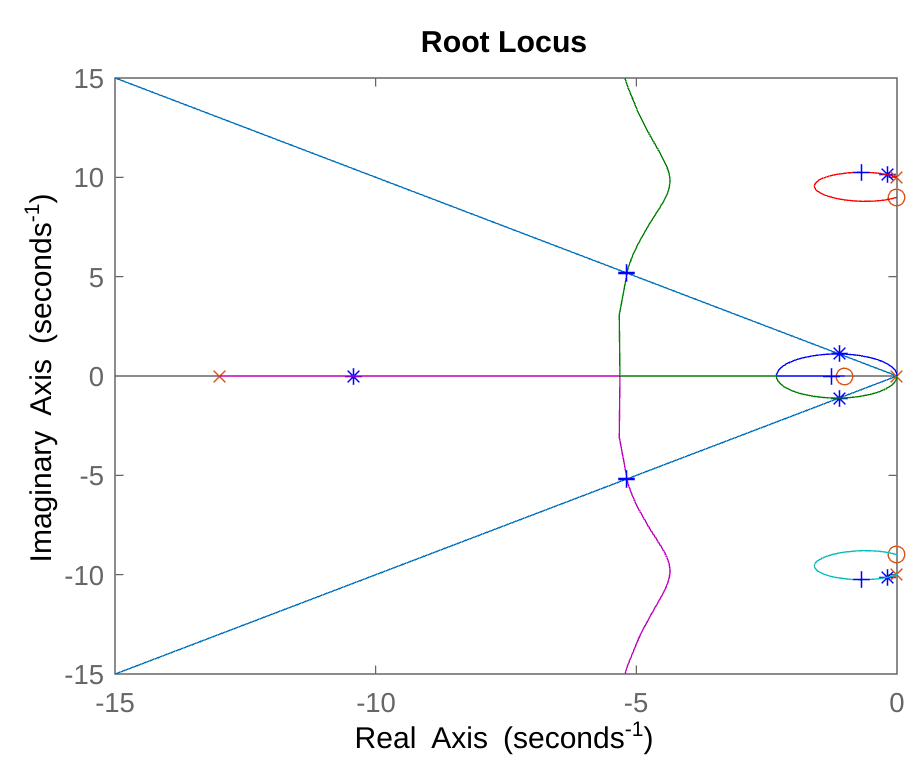
\includegraphics[scale=0.25]{Problem2Fig2.png}\\
With the points denoted with a $+$ sign being the poles from where $K=88.3$, and the points * are poles from where $K=32.6$
\subsection*{(d)}
Using the code below, we can plot the step response
\begin{verbatim}
syms s

G = tf([1 1 81 81],[1 13 100 1300 0 0]);

K=32.6;
sys=K*G/(1+K*G);

step(sys)
hold on;
K=88.3;
sys=K*G/(1+K*G);

step(sys)
hold off;
legend('K=32.6',"K=88.3")
\end{verbatim}
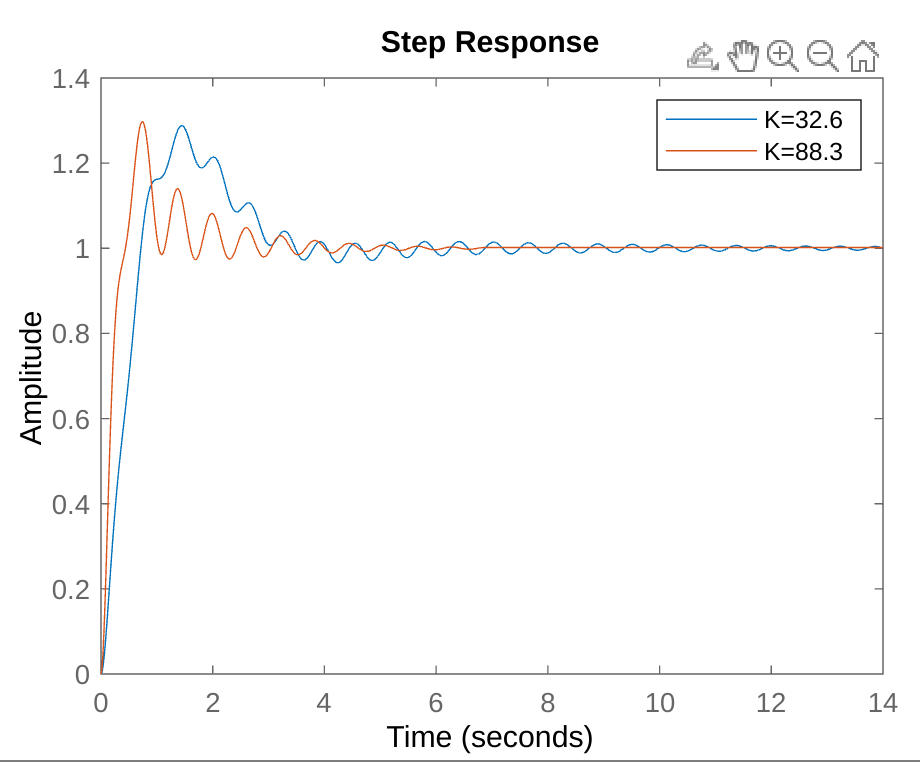
\includegraphics[scale=0.25]{Problem2Fig3.png}\\
\end{document}